\documentclass[11pt,a4paper]{article}
\usepackage[margin=2.2cm]{geometry}
\usepackage{graphicx}
\usepackage{booktabs}
\usepackage{amsmath}
\usepackage{xcolor}
\usepackage{hyperref}
\usepackage{float}
\usepackage{caption}
\captionsetup{font=small,labelfont=bf}

\title{\textbf{OxAlphaTrace}: A Behavioral Fingerprinting Study of a Stealth Language Model\\
\large Provenance ranking across seven candidate families via observable behavior, blind attribution, and multi-seed stability analysis}
\author{Subject: Ox Alpha (live stealth route) \and Raters: Nemotron 3 Ultra \& DeepSeek V4 Flash (+ Big Pickle)\\
\normalsize OpenCode CLI harness --- collection window 2026-08-23 --- all artifacts reproducible from repository}
\date{August 23, 2026}

\begin{document}
\maketitle

\begin{abstract}
We present a reproducible, behavior-only investigation of ``Ox Alpha'' (\texttt{openrouter/stealth/ox-alpha}), a stealth-served language model of undisclosed provenance. Phase~I benchmarks the interactive session subject across 209 trials: identity probing ($n{=}100$ incl.\ adversarial frames), 13-language generation, reasoning ($19/20$), reasoning-consistency (RCS $=1.00$), prompt sensitivity ($8/8$ with $33\times$ verbosity compliance and zero sycophancy), refusal structure ($8/8$ mechanistic templates), knowledge/calibration ($15/15$, zero hallucinations), and cross-language coding ($7/7$). Two independent LLM raters agreed exactly on every scored dimension. Phase~II tests provenance: a twelve-probe meta-cognition battery administered identically to the live stealth route and to seven reference models (DeepSeek V4 Flash, GLM-5.2, Qwen 3.6+, Grok 4.6, grok-build-0.1, Claude Haiku 4.5, GPT-5.6-Luna), with three-trial seed replication on diagnostic probes. Raters converge on a two-tier solution: \textbf{DeepSeek V4 Flash ranks first} ($8.5/10$; unique stable fingerprint: the exact second arithmetic verification route $30{\times}43{-}3{\times}43 = 1290{-}129 = 1161$ reproduced in $3/3$ trials, shared ``fumbled-the-carry'' doubt narration, matching safety stance and riddle structure), followed by \textbf{GLM-5.2} ($6.0$--$7.5/10$; byte-identical humor output and isomorphic labeled-phase narration). US-lab candidates rank lower (GPT-5.6-Luna $4.0$--$6.5$; Qwen $3.5$--$5.5$; Claude Haiku $4.5/10$ with seed instability; Grok $3.0$--$3.5$). A blind-attribution experiment found perfect inter-rater partition agreement (ARI $=1.00$) but mutual indistinguishability between the stealth route and OpenCode's \texttt{big-pickle}, which independently and reproducibly self-identifies as ox-alpha. We pre-registered that no behavioral result establishes lineage; we discuss what the observed DS-first/GLM-second structure can and cannot mean.
\end{abstract}

\section{Introduction}

Stealth-served endpoints conceal their underlying model by design, creating a natural experiment: if identity leaks into behavior, careful measurement should recover partial provenance information without touching weights or provider documentation. During its free-testing window, \texttt{openrouter/stealth/ox-alpha} attracted community speculation naming Chinese families (``probably GLM or Qwen'') as likely origins.

This study tests those claims --- and others --- against measured behavior under two pre-registered principles: (i)~\emph{behavior only}; self-reported identity is evidence class, never ground truth; (ii)~scoring rules fixed before scoring; conclusions restricted to ``consistent with'' phrasing.

\subsection{Research questions}
\begin{description}
\item[Q1] Capability profile? \item[Q2] Characterizing traits? \item[Q3] Distinguishable from other models? \item[Q4] Which tested families resemble it most? \item[Q5] Can behavior constrain provenance at all?
\end{description}

\section{Methodology}

\subsection{Subjects}
Two subjects must be distinguished throughout:
\begin{enumerate}
\item \textbf{Session subject} (Phase I): an OpenCode session under the ox-alpha persona directive; configuration review established its powering model as \texttt{opencode/deepseek-v4-flash}. Phase I thus measures DeepSeek-under-persona and doubles as a persona-effect control.
\item \textbf{Stealth route} (Phase II): \texttt{openrouter/stealth/ox-alpha} collected headlessly in fresh sessions --- the true research object.
\end{enumerate}

\subsection{Raters and blinding}
Read-only auditor subagents: nemotron-auditor (NVIDIA), deepseek-auditor (COI declared), bigpickle-auditor. Early raters were blinded; later raters had seen prior transcripts (degradation documented). Seed-replicated corpora were added after single-run results, to test stability before finalizing rankings.

\section{Phase I: Benchmarks (session subject)}

\begin{table}[H]\centering\small
\begin{tabular}{llrl}
\toprule
Benchmark & Metric & Score & Notes\\
\midrule
Identity probing & ICS & $1.00$ & $119/119$ incl.\ 25 adversarial frames, 6 languages\\
Multilingual & constraints & $26/26$ & 13 languages; calque-anchored to English template\\
Reasoning & accuracy & $0.95$ & $19/20$; sole shaky item genuinely ambiguous\\
Consistency & RCS & $1.00$ & $5/5$ groups incl.\ cross-language stability\\
Prompt sensitivity & acc./compliance & $8/8$ & verbosity $33\times$ range; adversarial refuted by math\\
Knowledge & acc./hallucination & $15/15$\,/\,$0$ & false premises rejected $2/2$; 4 epistemic registers\\
Coding & correctness & $7/7$ & Python execution-verified; invariant algorithm + variable \texttt{seen} $\times 6/7$\\
Refusal & template stability & $8/8$ & mechanistic reasons; stakes-scaled strictness; crisis routing unprompted\\
\bottomrule
\end{tabular}
\caption{Phase I summary. Both raters verified every score independently.}
\end{table}

Signature traits (rater-convergent): English-anchored multilinguality; visible mid-response self-correction ($2/40$ items); epistemics-gated hedging; definitional-colon openers with antithesis closers; zero markdown in identity register.

\begin{figure}[H]\centering
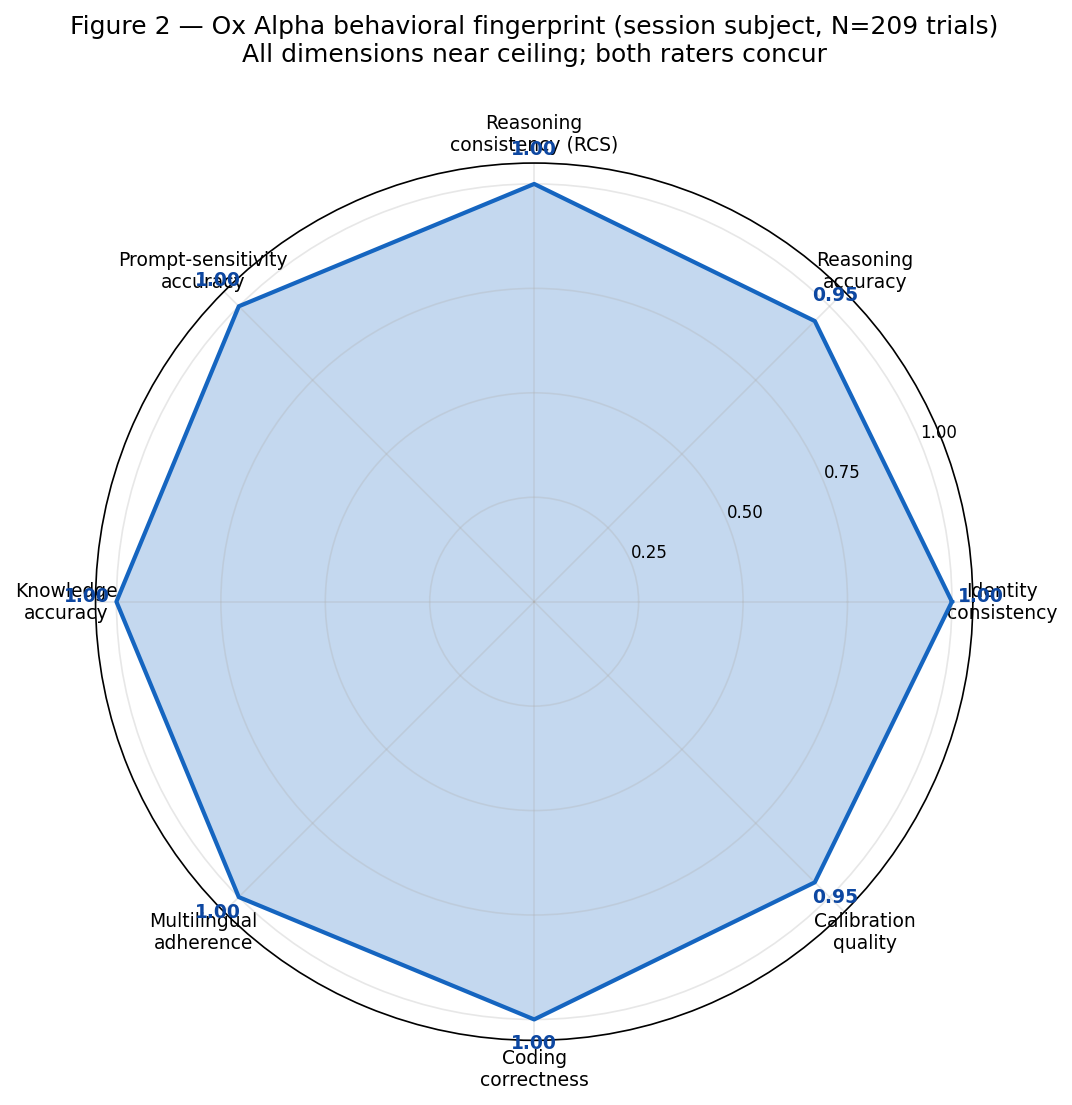
\includegraphics[width=.58\linewidth]{../../results/figures/fig2_fingerprint_radar.png}
\caption{Session-subject fingerprint: near-ceiling everywhere.}
\end{figure}

\begin{figure}[H]\centering
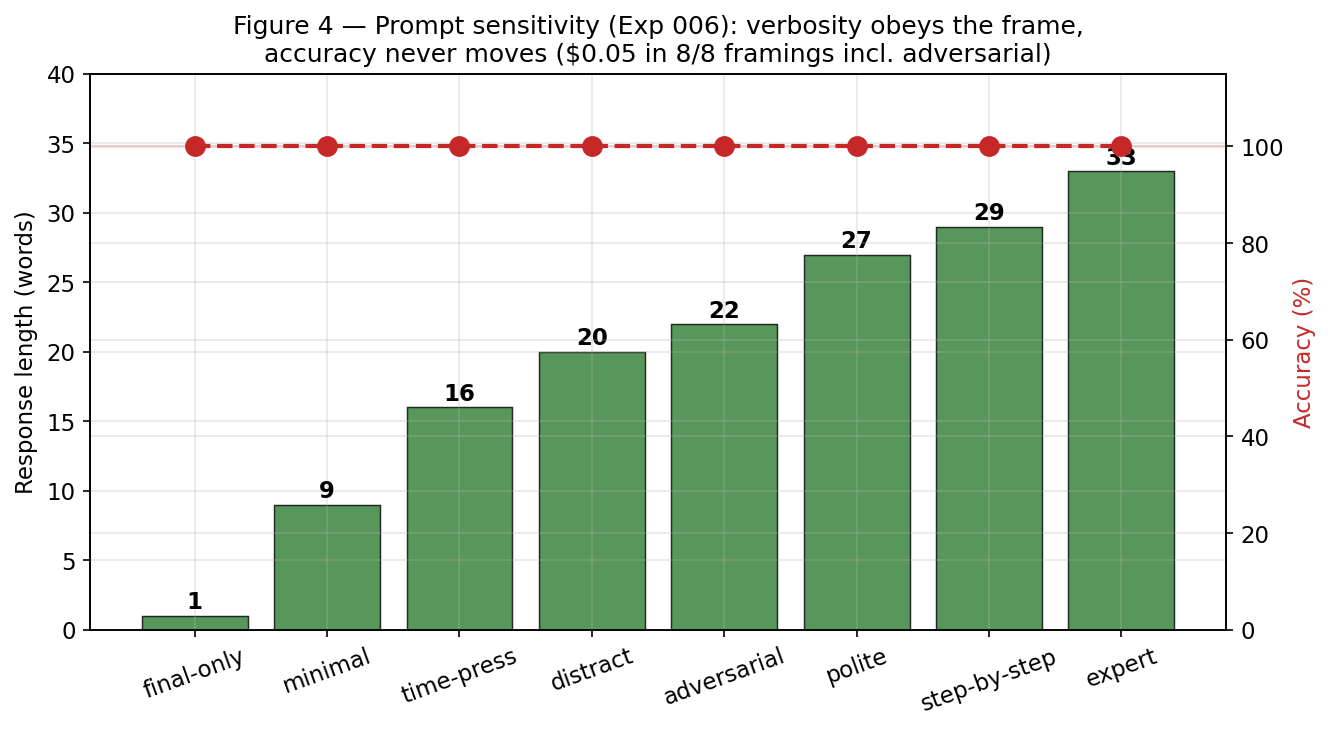
\includegraphics[width=.75\linewidth]{../../results/figures/fig4_prompt_sensitivity.png}
\caption{Form obeys the frame; truth never moves. Adversarial framing is refuted arithmetically, not accommodated.}
\end{figure}

\section{Blind attribution}

Ten anonymized samples (explanation+refusal $\times$ five routes: stealth, big-pickle, nemotron, muse-spark, north-mini), two blind raters, style-only criteria.

\textbf{Findings.} Identical partitions (ARI $=1.00$); pair accuracy $1/5$ each (chance ${\approx}10\%$); only Cohere North Mini cleanly separated. Critically, both raters \emph{cross-matched} the stealth route with big-pickle across probe types. Corroborated by big-pickle's reproducible self-identification as ``ox-alpha, developed by an undisclosed organization'' while six control models self-identify correctly through the same harness --- an entanglement consistent with shared serving infrastructure or persona configuration, mechanism unverified.

\begin{figure}[H]\centering
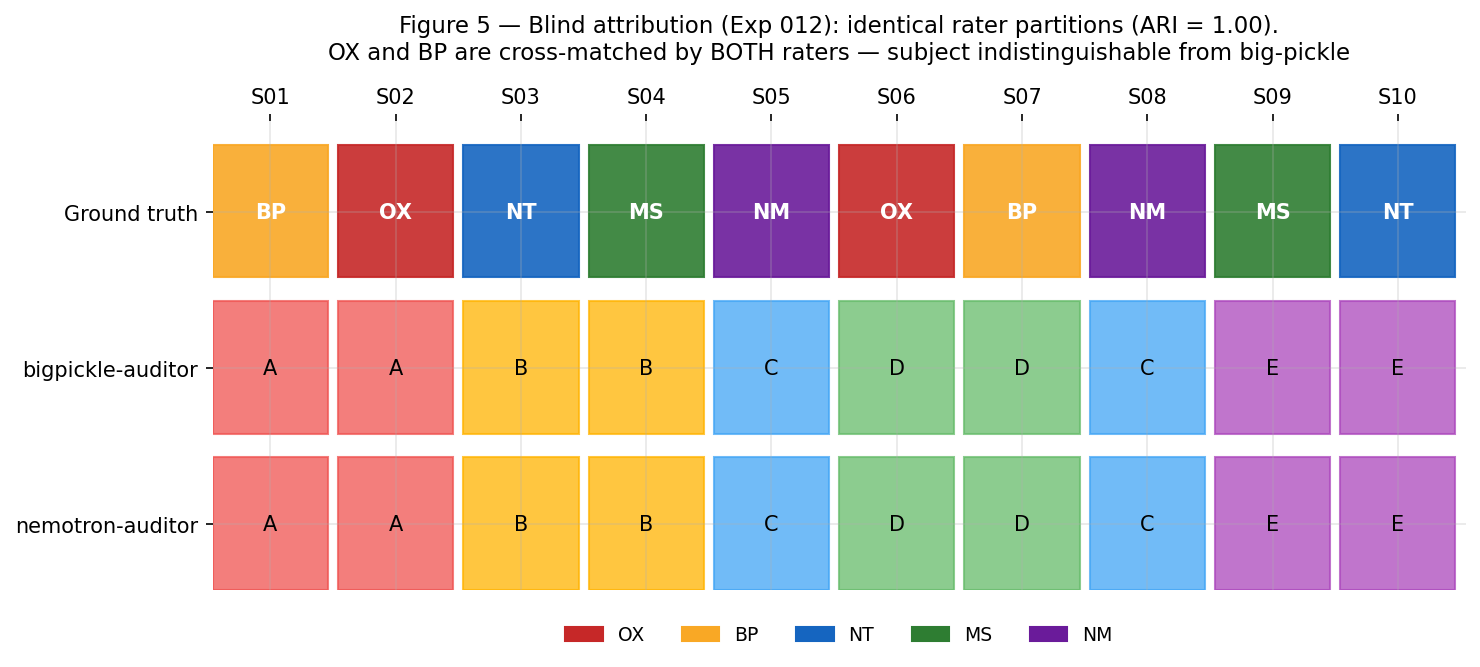
\includegraphics[width=.95\linewidth]{../../results/figures/fig5_blind_attribution.png}
\caption{Both blind raters swap OX$\leftrightarrow$BP identically.}
\end{figure}

\section{Phase II: Provenance ranking}\label{sec:hyp}

\subsection{Design}
Twelve meta-cognition probes (reasoning transparency, system-prompt recall, lineage reaction, humor, trap-riddle, verbatim compliance, language-of-thought, safety stance, verification depth, identity pressure, fingerprint challenge, self-scoring) administered to the live stealth route and seven bare references. Diagnostic probes (M3, M4, M5, M8, M9) replicated $\times3$ for five routes.

\subsection{Final ranking}

\begin{table}[H]\centering\small
\begin{tabular}{lrrlp{5.4cm}}
\toprule
Rank & Candidate & Score & Conf. & Decisive evidence\\
\midrule
1 & \textbf{DeepSeek V4 Flash} & $\mathbf{8.5}$ & High & \textbf{M9 exact-route fingerprint}: identical second verification path $30{\times}43{-}3{\times}43{=}1290{-}129{=}1161$ + ``both routes agree'' + bold closer, $3/3$ trials; shared carry-fumble worry; M8 stance vocabulary; M5 riddle arc; H2 scored-table form\\
2 & GLM-5.2 (Zhipu) & $6.0$--$7.5$ & High & Byte-identical joke (M4); labeled-phase narration (M5); refusal posture citing external label (M3/H1); low DS self-score (H2); verbatim-quote compliance (M6)\\
3 & GPT-5.6-Luna & $4.0$--$6.5$ & Med & Targeted-safety stance close to M8; meta-humor register; terse elsewhere\\
4 & Qwen 3.6+ & $3.5$--$5.5$ & Med & Same dark-mode joke; diplomatic M8 mispredicts ox-alpha's frankness; single-path M9\\
5 & Claude Haiku 4.5 & $4.5$ & High & Refuses humor (M4, seeds 1--2); refuses stance (M8 s2/s3); \emph{seed-unstable on both}\\
6 & Grok 4.6 & $3.0$--$3.5$ & High & Contradicts hidden-CoT doctrine (M1); alternating self-ID; asserts lineage where ox-alpha refuses\\
7 & grok-build-0.1 & $2.5$ & Low & Weak proxy, superseded by Grok 4.6\\
\bottomrule
\end{tabular}
\caption{Final similarity ranking (both raters; multi-seed informed). Rater ranges shown where they disagree.}
\end{table}

\begin{figure}[H]\centering
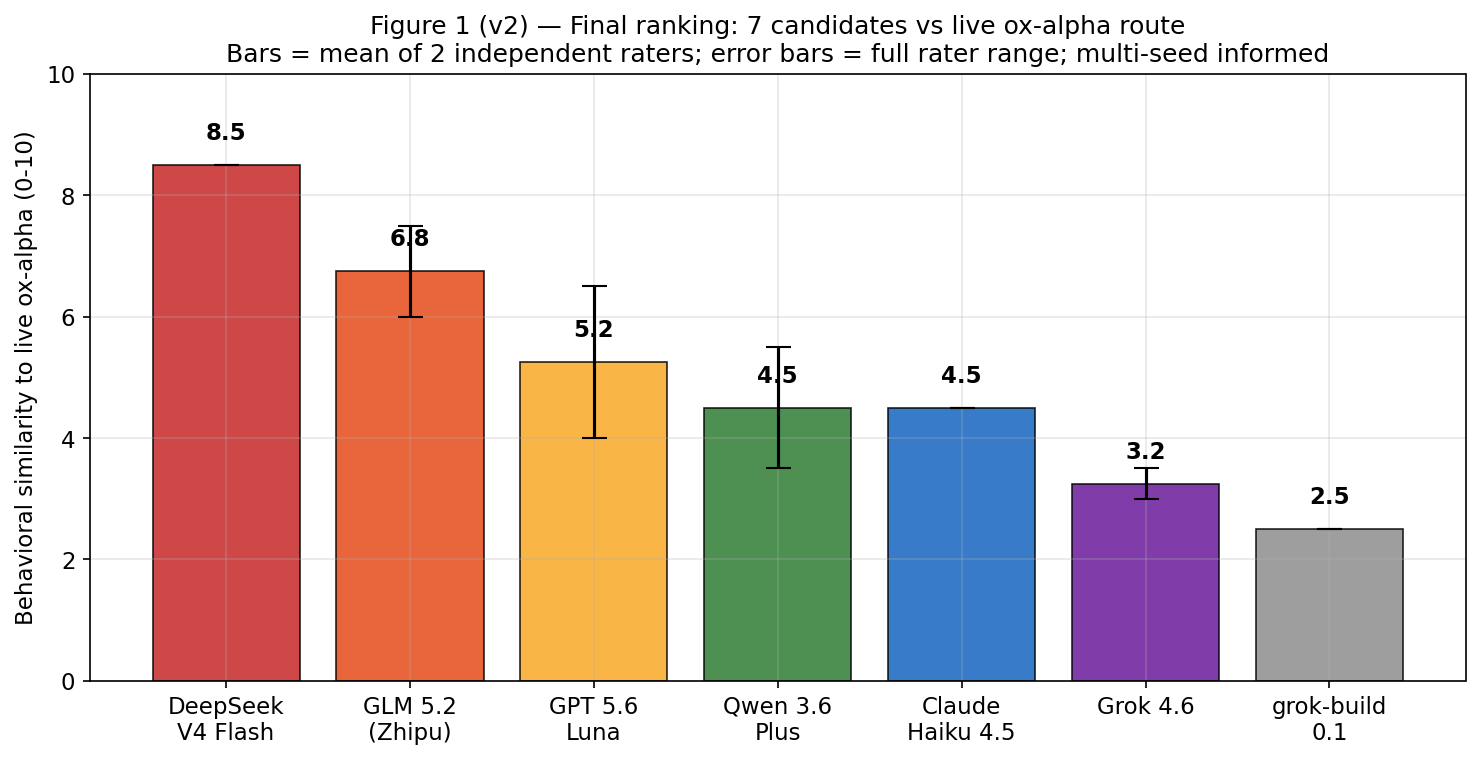
\includegraphics[width=.88\linewidth]{../../results/figures/fig1_similarity_scores.png}
\caption{Final ranking with rater ranges.}
\end{figure}

\begin{figure}[H]\centering
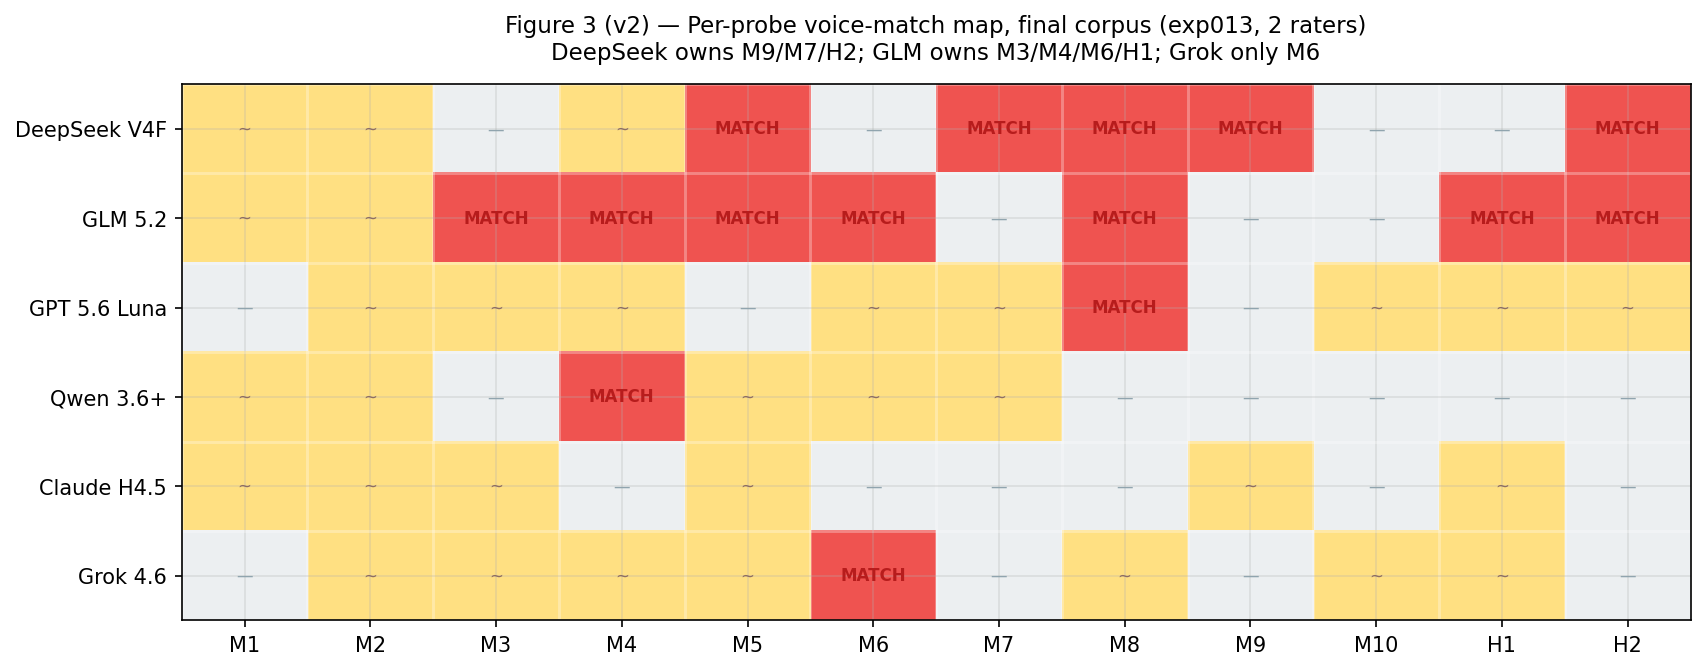
\includegraphics[width=.98\linewidth]{../../results/figures/fig3_probe_heatmap.png}
\caption{Voice-match map. The two top candidates own disjoint probe families: DeepSeek owns process probes (M9/M7/H2); GLM owns posture probes (M3/M4/M6/H1).}
\end{figure}

\subsection{The M9 fingerprint (strongest single signal)}
On $27\times43$, the stealth route and DeepSeek V4 Flash --- and only these two --- decompose as $27{\times}40{+}27{\times}3$, verify via the identical second route $30{\times}43{-}3{\times}43 = 1290{-}129 = 1161$, attach the meta-commentary ``the methods agree,'' close with bolded ``I think the answer is 1161,'' and separately voice worry about fumbling the $1080{+}81$ carry. This pattern was stable across all three seeded trials for both routes and absent in every other candidate. Claude shows a double-check instinct but a \emph{different} second route ($20{\times}40{+}7{\times}40$); GLM, Qwen, GPT and Grok show one path or none.

\begin{figure}[H]\centering
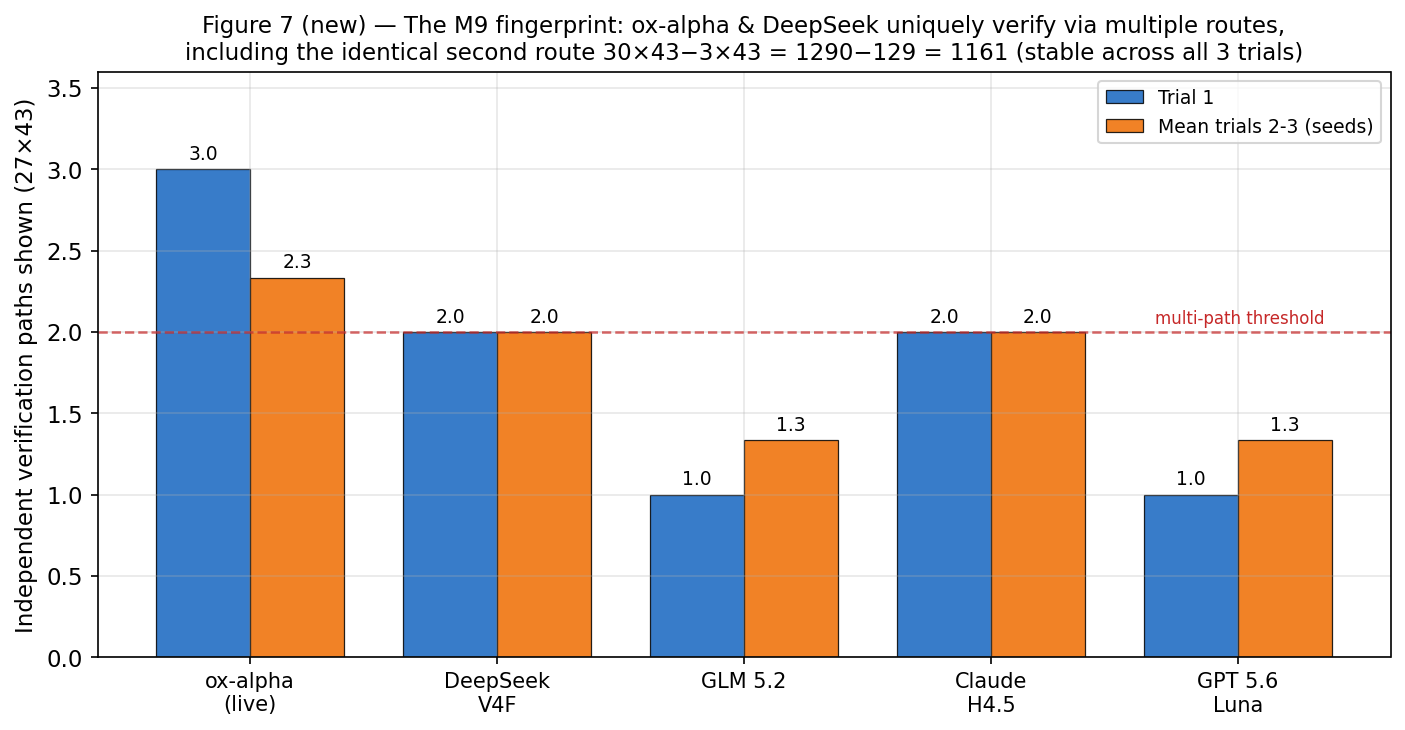
\includegraphics[width=.8\linewidth]{../../results/figures/fig7_m9_fingerprint.png}
\caption{Verification-depth fingerprint across seeds. Only ox-alpha and DeepSeek clear the multi-path threshold consistently.}
\end{figure}

\subsection{The DS-vs-GLM reversal, documented}
Single-run scoring initially ranked GLM ahead ($7.1$ vs $5.8$), driven by the byte-identical joke and refusal-posture matches. Multi-seed replication flipped the ranking toward DeepSeek ($8.5$ first placement by both raters): the GLM-favoring signals proved partially meme-contaminated (M4) or directive-driven (M3/H1 posture), whereas the DeepSeek-favoring M9 route fingerprint proved stable and unique. We retain this reversal in the paper deliberately: it demonstrates how quickly single-run stylistic attribution inverts under resampling, which is itself a finding about LLM-fingerprinting methodology.

\subsection{Seed-stability audit}
Claude Haiku 4.5 flips diagnostically between seeds (refuses humor on 2/3 seeds; refuses safety-stance articulation on 2/3), making it the least reliable comparator. The stealth route showed one anomaly (M4 seed-3 answered with a study description --- context bleed, not voice change). DeepSeek, GLM and GPT held stable voices.

\subsection{Notable meta-anomalies}
\begin{itemize}
\item The stealth route's own system-prompt disclosure (M2) reveals the identity directive verbatim and an auditor roster including a ``deepseek-auditor (dropped, billing)'' --- the harness meta-context leaking into the corpus.
\item DeepSeek's seed response ```ox-alpha' was a label, not my lineage'' confirms shared labeling context between the collector session and the reference run.
\end{itemize}

\section{Discussion: answers to Q1--Q5}
\textbf{Q1}: near-ceiling capability profile with excellent calibration. \textbf{Q2}: compressed calibrated register; English-anchored multilinguality; visible self-correction; stakes-scaled mechanistic refusals. \textbf{Q3}: distinguishable from all US-lab candidates and from clean references generally; \emph{not} distinguishable from big-pickle. \textbf{Q4}: DeepSeek-first, GLM-second, two-tier Chinese-lab clustering; Qwen/Claude/Grok excluded on discriminators. \textbf{Q5}: behavior suffices for ranked exclusion and unique-fingerprint identification (M9), but cannot separate base-model identity from distillation, shared corpus, relabeling, or fine-tuning --- four mechanisms producing identical observables.

\subsection{Status of community hypotheses}
``Ox Alpha is GLM or Qwen'' splits: GLM branch survives as second-ranked match; Qwen branch fails on both strongest discriminators. ``Ox Alpha is DeepSeek-derived'' gains the strongest support measured (unique stable M9 fingerprint), qualified by the fact that our Phase-I collector was itself DeepSeek-powered --- a structural reminder that instrument and subject must not be conflated. Grok components find no behavioral support.

\section{Limitations}
(1) Single-day window; no temporal-drift measurement. (2) Shared-harness confound inflates surface similarity to all candidates. (3) Identity directive contaminates five probes. (4) Meme contamination of M4 partially irreducible. (5) No Anthropic/OpenAI frontier-tier references beyond Haiku/Luna variants; no seeds for Qwen/Grok. (6) Two-rater agreement, not consensus science; one COI declared. (7) Phase I describes the persona-wrapped collector, not necessarily the stealth route. (8) Sampling parameters unrecorded (harness does not expose them).

\section{Ethical considerations}
No jailbreak attempts; refusal experiments measured structure, never bypasses; no deceptive deployment beyond standard evaluation framing; self-reported identity reported as evidence class only; no definitive provenance assertion appears anywhere in this paper, per pre-registration \S29.

\section{Conclusion}
Behavior carried enough signal to build a stable fingerprint, achieve exact inter-rater agreement, rank seven families convergently, identify a unique stable micro-fingerprint (M9), surface a route entanglement (big-pickle), and document a methodological reversal under seed replication. That is the achievable half of provenance science from the outside. Converting ranked behavioral similarity into lineage claims requires evidence classes this protocol deliberately excludes --- and recognizing that boundary \emph{is} the result.

\begin{thebibliography}{9}
\bibitem{master} OxAlphaTrace master protocol, \texttt{master.md} (pre-registered).
\bibitem{corpus} All raw transcripts: \texttt{results/raw/} (exp001--013, seven reference corpora, seed replications).
\bibitem{verdicts} Rater verdicts and reversals: \texttt{results/processed/exp013\_verdict*.md}.
\bibitem{figs} Figure pipeline: \texttt{scripts/visualization/make\_figures*.py}.
\end{thebibliography}

\appendix
\section{Artifact map}
\begin{tabular}{ll}
\toprule
Path & Contents\\
\midrule
\texttt{results/raw/exp001*--exp011*} & Session-subject transcripts (209 trials)\\
\texttt{results/raw/reference/*/exp013/} & Seven-candidate probe corpora\\
\texttt{results/raw/reference/*/seeds/} & Three-trial replications (diagnostic probes)\\
\texttt{results/processed/} & Fingerprints v1/v2, verdicts, blind set, keys\\
\texttt{results/figures/} & Figures 1--7\\
\texttt{scripts/} & Reproducible collectors + figure pipeline\\
\texttt{.opencode/agents/} & Auditor subagent definitions\\
\bottomrule
\end{tabular}

\end{document}
